\documentclass[
	classe=$1^{ere}$STI2D,
	exercices=Images\space et\space antécédents,
	noheader
]{exercice}

\usepackage{clipboard}

\title{Images et antécédents}

\newcommand{\makegrid}[2]{
	\foreach \y in {-#1, ..., #1} {
		\draw[ultra thin] (-#2,\y) -- (#2,\y);
		\ifthenelse{\equal{\y}{0}}{}{
		\draw[thick] (-0.2,\y) node[left] {\y} -- (0,\y);
		}
	}
	\foreach \x in {-#2, ..., #2} {
		\draw[ultra thin] (\x,-#1) -- (\x,#1);
		\ifthenelse{\equal{\x}{0}}{}{
		\draw[thick] (\x,-0.2) node[below] {\x} -- (\x,0);
		}
	}
	\node[below,left] at (-0.2,-0.3) {$0$};
	\draw[very thick,\myArrow] (-#2 - 0.3,0) -- (#2 + 0.5,0);
	\draw[very thick,\myArrow] (0,-#1 - 0.3) -- (0,#1 + 0.5);
}

\begin{document}

\Copy{exos}{
	\maketitle

	\textbf{\uline{Exercice 3}.}
	Soit $h$ la fonction qui à $x$ associe $\dfrac{x}{2} + 3$. \vspace{1em}

	\begin{minipage}{0.35\linewidth}
		Déterminer :
		\begin{itemize}
			\item l'image de $6$ par $h$ : \correction{$6$}
			\item l'image de $2$ par $h$ : \correction{$4$}
			\item l'image de $3$ par $h$ : \correction{$4,5$}
			\item l'image de $-4$ par $h$ : \correction{$1$}
			\item Un antécédent de $3$ par $h$ : \correction{$0$}
			\item Un antécédent de $-0,5$ par $h$ : \correction{$-7$}
		\end{itemize}
	\end{minipage}
	\hfill\vrule\hfill
	\begin{minipage}{0.55\linewidth}
		Placer les points obtenus sur le graphe suivant :\vspace{1em}

		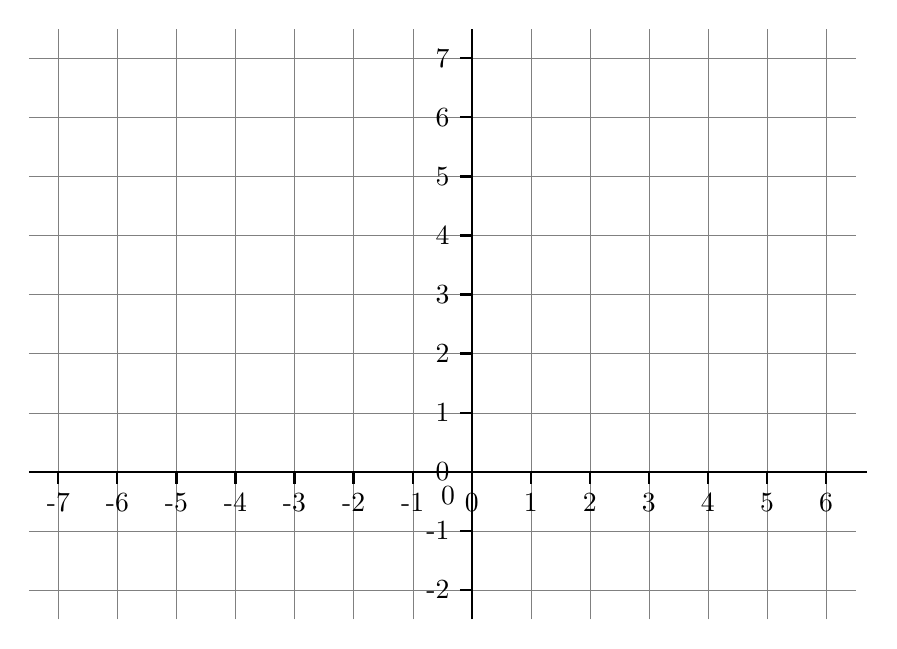
\begin{tikzpicture}[scale=0.75]
			\draw[ultra thin,gray] (-7.5,-2.5) grid (6.5,7.5);
			\draw[thick,\myArrow] (-7.5,0) -- (6.7,0);
			\draw[thick,\myArrow] (0,-2.5) -- (0,7.5);

			\foreach \y in {-2, ..., 7} {
					\ifthenelse{\equal{\y}{0}}{}{
						\draw[thick] (-0.2,\y) node[left] {\y} -- (0,\y);
					}
				}
			\foreach \x in {-7, ..., 6} {
					\ifthenelse{\equal{\x}{0}}{}{
						\draw[thick] (\x,-0.2) node[below] {\x} -- (\x,0);
					}
				}
			\node at (-0.4,-0.4) {0};

			\ifdefined\makeCorrection
				\foreach \x/\y in {6/6,2/4,3/4.5,-4/1,0/3,-7/-0.5} {
						\node[red] at (\x,\y) {×};
					}
			\fi
		\end{tikzpicture}
	\end{minipage}
}

\vspace{5em}

\Paste{exos}


\end{document}